\documentclass[12pt, a4paper]{book}

\usepackage{fancyhdr}
\usepackage[left=4cm, right=4cm, top=4cm, bottom=4cm]{geometry}
\usepackage[utf8]{inputenc}
\usepackage[table]{xcolor}
\usepackage{hyperref}
\usepackage{amsmath}
\usepackage{enumitem}
\usepackage{graphicx}
\usepackage{amsfonts}
\usepackage{booktabs}
\usepackage{subcaption}
\usepackage[justification=centering]{caption}
\usepackage{xepersian}

\DeclareMathOperator*{\argmax}{argmax}
\DeclareMathOperator*{\argmin}{argmin}
\newcolumntype{L}{>{$}l<{$}} % math-mode version of "l" column type

\newcommand{\coursetitle}{فهم زبان طبیعی}
\newcommand{\doctitle}{تمرین دوم}
\newcommand{\name}{محمدرضا غفرانی}
\newcommand{\studentno}{400131076}
\newcommand{\todaydate}{\today}

\settextfont{XB Kayhan}
\setlatintextfont{Times Newer Roman}

\pagestyle{fancy}
\rhead{\name}
\lhead{\textbf{\doctitle}}

\begin{document}

\begin{flushleft}
    \name \\
    \studentno \\
    \todaydate
\end{flushleft}

\begin{center}
    \huge
    \textbf{\coursetitle}
    \break
    \large
    \doctitle
\end{center}

% suppress the fancy header on the first page only
\thispagestyle{plain}

\section*{ساختار پروژه}

% توضیحات کلی در رابطه با ورودی‌ها و خروجی‌ها

برای انجام این پروژه از مدل‌های \lr{T5} و \lr{BERT} که مبتنی بر شبکه‌های \lr{transformer} هستند،
استفاده شده است. مدل \lr{T5} هر دو قسمت کدگذار و کدگشای \lr{transformer} را در بر دارد،
اما مدل \lr{BERT} تنها شامل قسمت کد‌گذار ساختار \lr{transformer} است. در ادامه در بخش‌های متناظر
در رابطه با جزئیات پیاده‌سازی هر کدام از شبکه‌ها و نحوه فرمول‌سازی ورودی و خروجی بیشتر توضیح داده می‌شود.

‌مجموعه‌داده‌ای که در این تمرین در اختیار ما قرار گرفته بود بر پایه ساختار \lr{conllu} بود. این ساختار
به گونه‌ای است که می‌تواند هم جمله ورودی و هم خروجی‌ها که شامل اسلات‌\LTRfootnote{slot}ها و قصد\LTRfootnote{intent} کاربر است را در یک فایل
نمایش دهد. ما با انجام یک پیش‌پردازش مختصر، ورودی‌ها و خروجی‌ها به سه فایل مجزا تقسیم کرده‌ایم.
یکی از این فایل‌ها (\lr{seq\_in}) تنها شامل جمله ورودی،
فایل دیگر (\lr{seq\_out}) شامل دنباله اسلات‌ها و فایل سوم (\lr{labels}) قصد کاربر از بیان
هر جمله است. کد مربوط به این پیش‌پردازش در فایل \lr{preprocess.py} قرار گرفته است.

\section*{مدل \lr{BERT}}

% پیاده‌سازی انجام شده
% توضیحات ورودی‌ها و خروجی‌ها
% شیوه هندل‌کردن شکسته‌شدن توکن‌ها
% نوآوری‌ها

مدل \lr{BERT} یک مدل کدگذار است و برای هر کلمه ورودی یک بردار بازنمایی خروجی می‌دهد. با توجه به این
موضوع ما پس از دریافت بردار بازنمایی متناظر هر کلمه، بردار را به یک شبکه عصبی یک لایه می‌دهیم تا
کار دسته‌بندی شکاف را برای ما انجام دهد. برای تشخیص قصد کاربر از توکن \lr{[CLS]} که در مدل \lr{BERT}
به منظور نشان دادن ابتدای عبارت استفاده می‌شود بهره می‌گیریم. به صورت مشابه بردار بازنمایی متناظر
این کلمه به یک شبکه عصبی یک لایه داده می‌شود تا دسته‌بندی قصد کاربر انجام شود. در \autoref{bert_architecture}،
توضیحات بیان شده به صورت تصویری مشاهده می‌شود.

نکته‌ای که در مدل \lr{BERT} باید به آن توجه کرد مسئله شکسته‌شدن یک کلمه به زیر کلمه‌هاست. همان‌طور که می‌دانید
توکن‌کننده مدل \lr{BERT} هر کلمه ورودی را ممکن است به زیرکلمه‌های آن بشکند. این شکسته‌شدن باعث می‌شود که
یک بردار بازنمایی آن کلمه در خروجی نباشد، بلکه برای به دست آوردن بردار متناظر کلمه باید از روش‌هایی نظیر
میانگین‌گیری بردار زیرکلمه‌ها، الحاق بردار‌های زیرکلمه به یکدیگر و غیره استفاده کرد. ما در این این جا برای سادگی
بردار متناظر اولین زیرکلمه را به عنوان بردار معرف آن کلمه در نظیر گرفته و بر اساس آن عملیات دسته‌بندی
شکاف‌ را انجام می‌دهیم. باقی زیرکلمه‌ در این حالت نادیده گرفته شده و با \lr{<pad>} نمایش داده می‌شود.
این مطلب در \autoref{bert_architecture} نیز دیده می‌شود.

\begin{figure}[h]
    \centering
    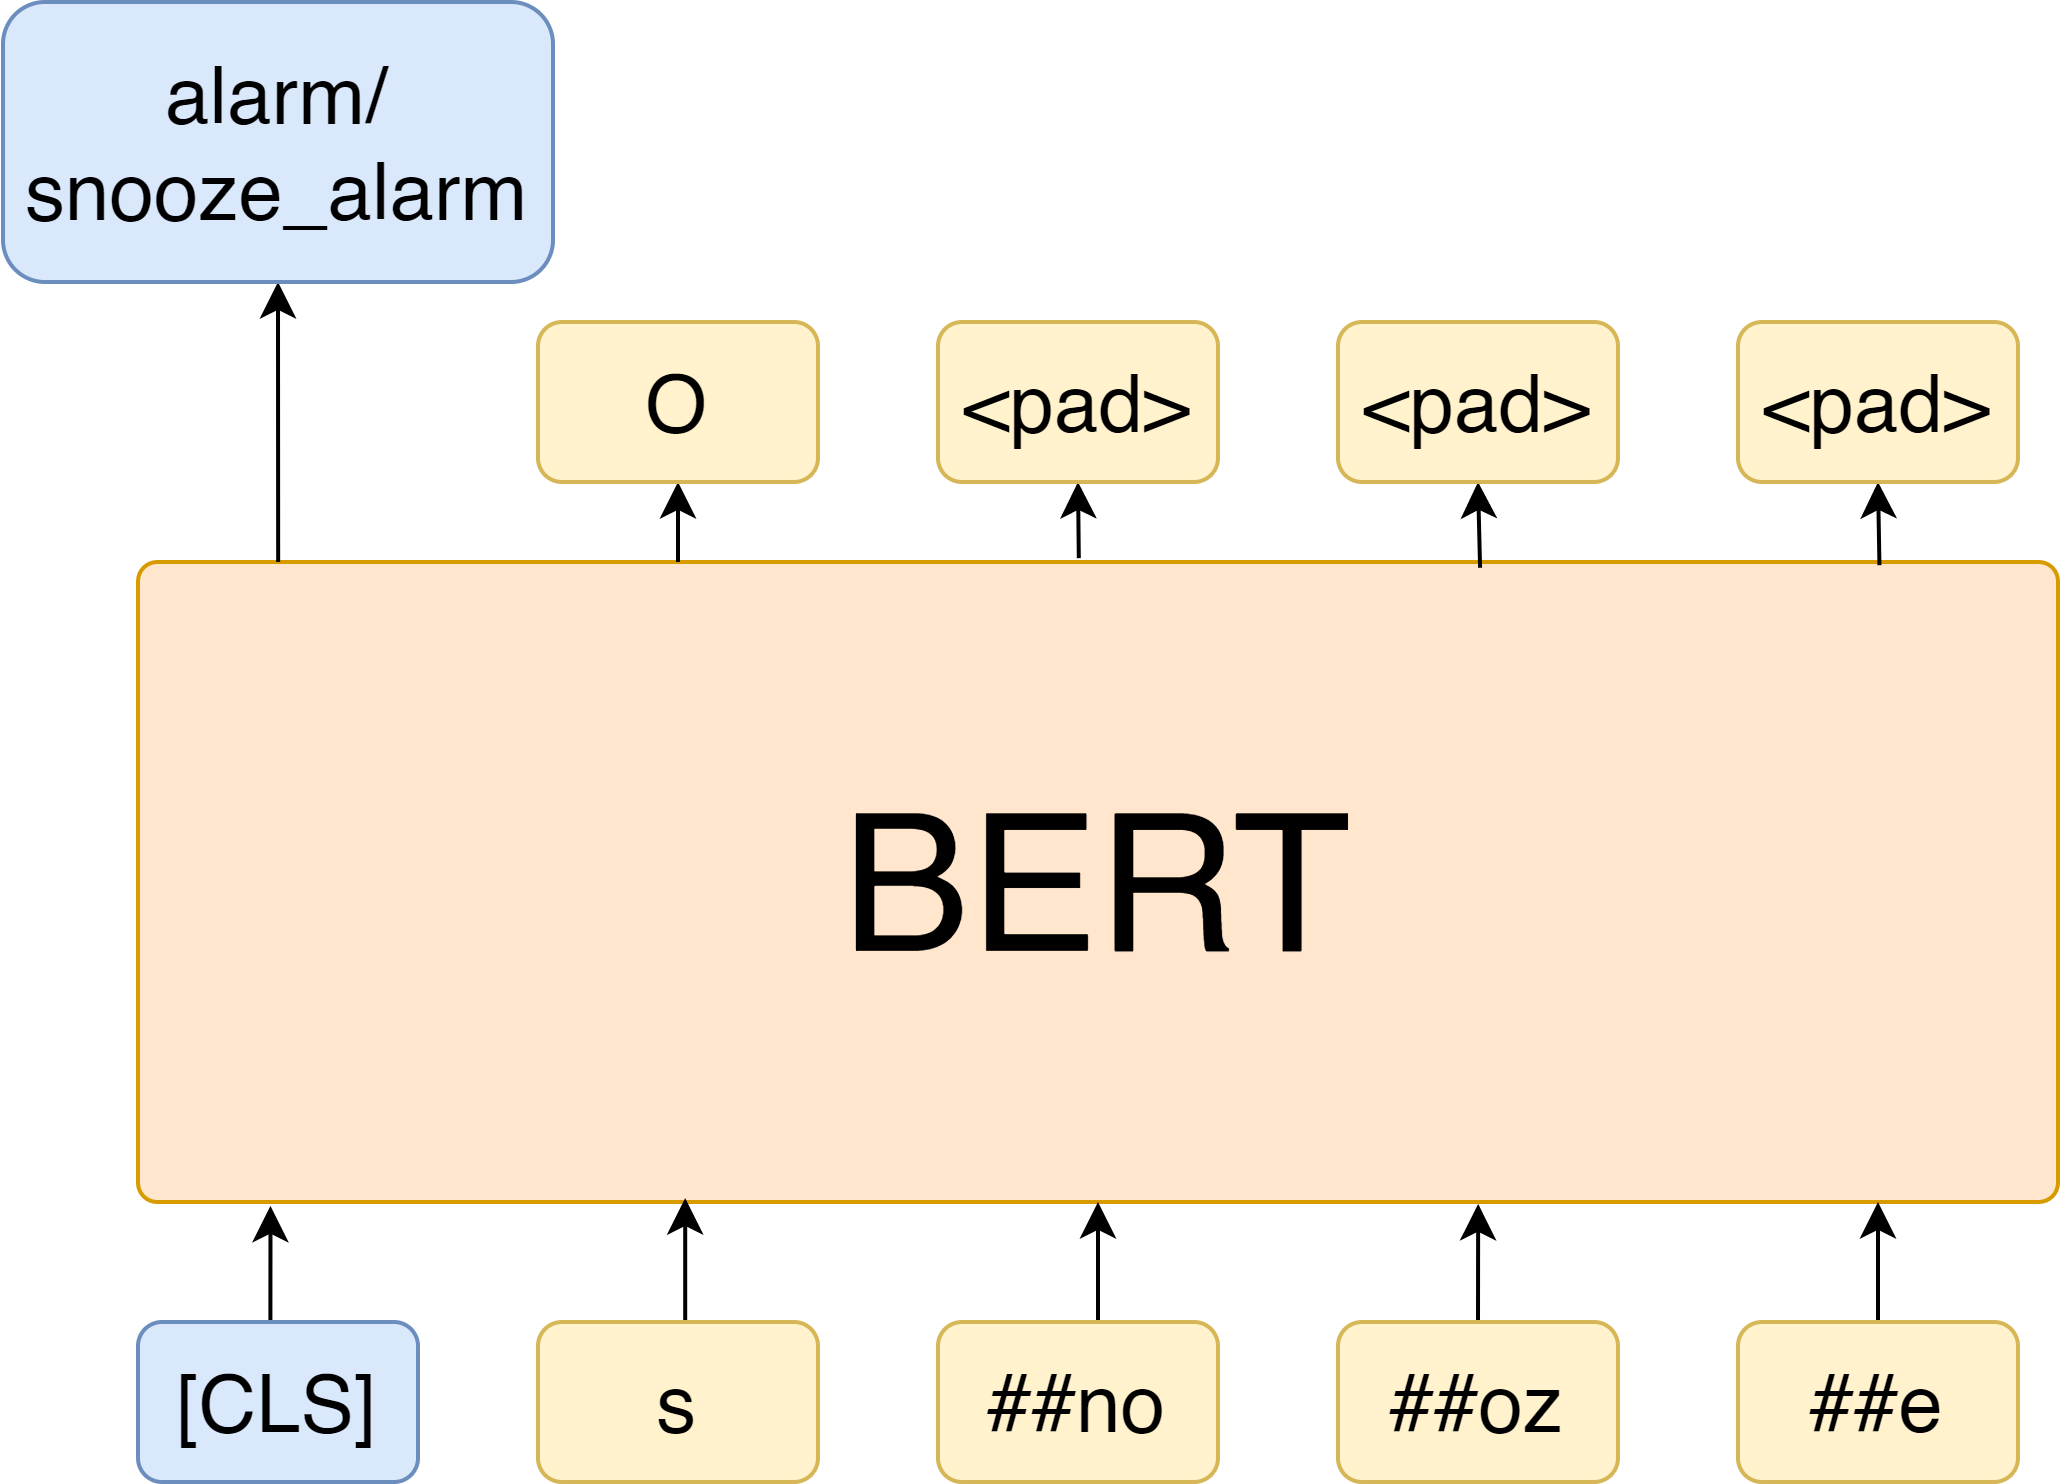
\includegraphics[width=0.5\linewidth]{images/bert/architecture.png}
    \caption{نحوه استفاده از مدل \lr{BERT} برای تشخیص قصد و پرکردن شکاف}
    \label{bert_architecture}
\end{figure}

در \autoref{bert_loss} تغییرات خطای مدل در هنگام آموزش در داده‌های آموزشی و ارزیابی مشاهده می‌شود.
با توجه به این نمودار مدل دچار بیش‌برازش نشده است. لازم به ذکر است که برای جلوگیری از بیش‌برازش
از تکنیک \lr{drop-out} با نرخ $0.1$ نیز استفاده شده است. به علاوه در هنگام یادگیری مدل ضریب یادگیری
برابر $5 \times 10^{-5}$ در نظر گرفته شده است.

\begin{figure}[h]
    \centering
    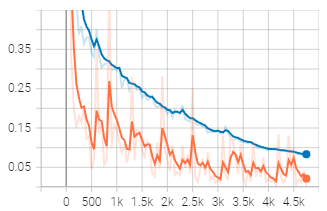
\includegraphics[width=0.5\linewidth]{images/bert/loss.png}
    \caption{تغییرات خطا مدل در هنگام آموزش. نمودار آبی میزان خطای در داده‌های ارزیابی و نمودار نارنجی‌رنگ خطا در داده‌های آموزشی را نشان می‌دهد. }
    \label{bert_loss}
\end{figure}

عملکرد مدل \lr{BERT} به ازای تنظیمات مختلف در \autoref{bert_results} آورده شده است.
برای بهبود عملکرد مدل \lr{BERT} و انتخاب بهتر خروجی‌ها از مدل \lr{CRF}\LTRfootnote{Conditional random field}
در هنگام کدگشایی مدل نیز استفاده شده است. استفاده از این مدل باعث بهبود عملکرد مدل \lr{BERT} شده است.

\begin{table}[h]
    \centering
    \caption{نتایج عملکرد مدل \lr{BERT} به ازای تنظیمات مختلف}
    \label{bert_results}
    \setLTR
    \begin{tabular}{c|c|c|c|c}
        & \multicolumn{3}{c|}{شکاف} & \multicolumn{1}{c}{قصد} \\
        \hline
        توضیحات & بازیابی & دقت & F1 & صحت \\
        \hline
        \lr{dropout=0.1} \& \lr{lr=$5 \times 10^{-5}$} \& \lr{no crf} & $96.31$ & $95.86$ & $96.09$ & $99.47$ \\
        \lr{dropout=0.1} \& \lr{lr=$5 \times 10^{-5}$} \& \lr{crf} & $96.35$ & $96.14$ & $96.24$ & $99.37$ \\
        \lr{dropout=0.1} \& \lr{lr=$10^{-5}$} \& \lr{crf} & $96.5$ & $95.8$ & $96.15$ & $98.71$ \\
        \lr{dropout=0.2} \& \lr{lr=$10^{-5}$} \& \lr{crf} & $96.47$ & $95.78$ & $96.12$ & $98.67$ \\
    \end{tabular}
\end{table}


\section*{مدل \lr{T5}}

% پیاده‌سازی انجام شده
% توضیحات ورودی‌ها و خروجی‌ها
% شیوه هندل‌کردن شکسته‌شدن توکن‌ها
% نوآوری‌ها
% *بازنمایی بهتر خروجی*: خروجی گرفتن تنها آن قسمت از ورودی که مدل نظر است.

برخلاف مدل \lr{BERT}، مدل \lr{T5} هم شامل قسمت کدگذار و هم شامل قسمت کدگشای مدل \lr{transformer} است.
از آن جا که هم ورودی و هم خروجی مدل \lr{T5} باید به صورت متن باشد، بنابراین پیش‌پردازشی
روی متن خروجی انجام نمی‌شود و تنها وظیفه مورد انتظار به جمله ورودی اضافه می‌شود.
در \autoref{t5_architecture} نمونه انجام این کار آورده شده است.

\begin{figure}[h]
    \centering
    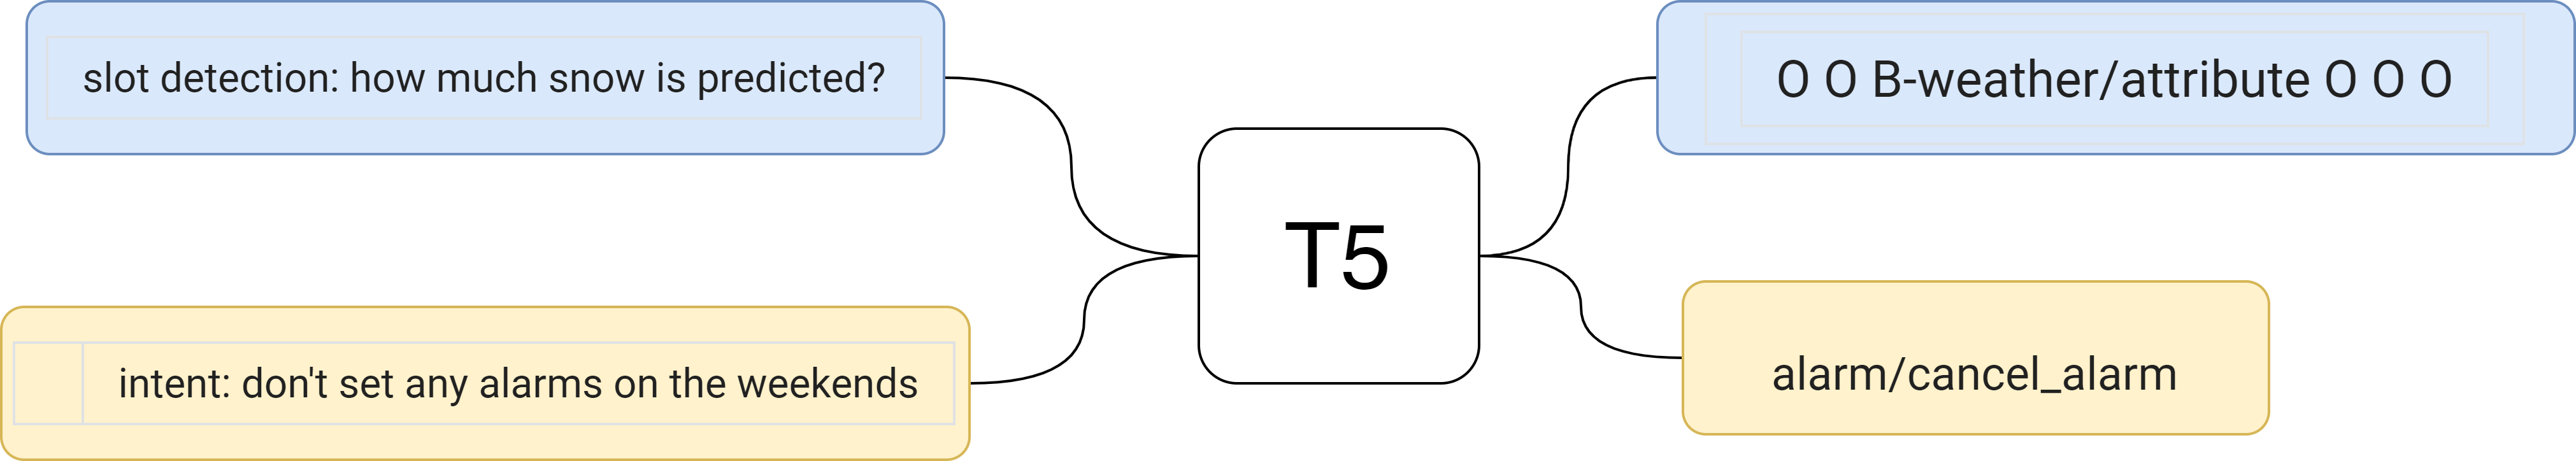
\includegraphics[width=0.8\linewidth]{images/t5/architecture.png}
    \caption{نحوه استفاده از مدل \lr{T5} برای تشخیص قصد و پرکردن شکاف}
    \label{t5_architecture}
\end{figure}

در \autoref{t5_loss} میزان تغییرات خطای مدل در هنگام آموزش را نشان می‌دهد. در این نمودار مدل به تعداد
۵ گام یادگیری، آموزش دیده است. همان‌طور که مشخص است در گام‌های نهایی خطای مدل تقریبا به صفر رسیده است.
بر طبق این نمودار مدل بر روی داده‌های آموزشی دچار بیش‌برازش نشده است.

\begin{figure}[h]
    \centering
    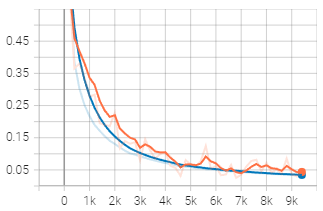
\includegraphics[width=0.5\linewidth]{images/t5/loss.png}
    \caption{تغییرات خطای مدل \lr{T5} در هنگام آموزش. نمودار آبی میزان خطای در داده‌های ارزیابی و نمودار نارنجی‌رنگ خطا در داده‌های آموزشی را نشان می‌دهد. }
    \label{t5_loss}
\end{figure}

در \autoref{t5_results} نتایج مربوط به مدل \lr{T5} مشاهده می‌شود. برای رسیدن به این نتایج
مدل به تعداد ۵ گام آموزش دیده است. این عملکرد در مقایسه با عملکرد مدل
\lr{BERT} در \autoref{bert_results} ضعیف‌تر است. در قسمت بعدی در رابطه با علت این اتفاق بیشتر بحث خواهیم کرد.

\begin{table}[h]
    \centering
    \caption{نتایج عملکرد مدل \lr{T5} به ازای تنظیمات مختلف}
    \label{t5_results}
    \setLTR
    \begin{tabular}{c|c|c|c|c}
         & \multicolumn{3}{c|}{شکاف} & \multicolumn{1}{c}{قصد} \\
        \hline
        توضیحات & بازیابی & دقت & F1 & صحت \\
        \hline
        \lr{lr=$5 \times 10^{-5}$} & $79.72$ & $72.18$ & $75.76$ & $99.08$ \\
    \end{tabular}
\end{table}

در ادامه برخی از پیش‌پینی‌های انجام شده توسط مدل \lr{T5} به همراه خروجی‌های مورد انتظار آورده شده است.

\begin{latin}
    \begin{itemize}
        \item cancel my reminder at 7 : 00.
        \begin{enumerate}
            \item Ground Truth Slot: O O B-reminder/noun B-datetime I-datetime I-datetime I-datetime O
            \item Predicted Slot: O O B-reminder/noun B-datetime I-datetime I-
            \item Ground Truth Intent: reminder/cancel\_reminder
            \item Predicted Intent: reminder/cancel\_reminder
        \end{enumerate}
        \item how much snow is predicted?
        \begin{enumerate}
            \item Ground Truth Slot: O O B-weather/attribute O O O
            \item Predicted Slot: O O B-weather/attribute O O O
            \item Ground Truth Intent: weather/find
            \item Predicted Intent: weather/find
        \end{enumerate}
        \item set 2 alarms for tomorrow
        \begin{enumerate}
            \item Ground Truth Slot: O O O B-datetime I-datetime
            \item Predicted Slot: O O O B-datetime I-datetime
            \item Ground Truth Intent: alarm/set\_alarm
            \item Predicted Intent: alarm/set\_alarm
        \end{enumerate}
    \end{itemize}
\end{latin}

\section*{مقایسه‌ مدل‌ها}

در این تمرین از دو مدل \lr{T5} و \lr{BERT} برای انجام وظیفه تشخیص قصد و پر کردن شکاف
استفاده کرده‌ایم. با توجه به نتایج، عملکرد مدل \lr{BERT} برای انجام این وظایف بسیار بهتر از
عملکرد مدل \lr{T5} است، چرا که مدل \lr{BERT} با توجه به نحوه آموزش و نحوه گرفتن ورودی‌ها و خروجی‌ها
به گونه‌ای است که بسیار منطبق بر وظیفه محول شده است. در مقابل مدل \lr{T5} گرچه در انجام
وظیفه پرکردن شکاف نتوانسته به خوبی عمل کند اما وظیفه تشخیص قصد کاربر را به خوبی و با صحت ۹۹ درصد
انجام داده است. وظیفه پر کردن شکاف در فرمول‌بندی که ما برای ورودی‌ها و خروجی‌های مدل \lr{T5}
انجام داده بودیم، برای مدل \lr{T5} کار سختی بود. چرا که مدل \lr{T5} در هنگام آموزش بر روی داده‌های زبان
طبیعی و جملات آن آموزش دیده است اما خروجی که ما از مدل انتظار داریم رشته‌ای (تقریبا بی‌معنی) از
برچسب‌هاست. در این فرمول‌بندی مدل خود باید متوجه بشود که باید دنباله‌ای از برچسب‌ها دریافت می‌کند و
در نتیجه باید با استفاده از کاراکتر فاصله آن‌ها را از یکدیگر تمییز دهد و سپس در ادامه باید
متوجه شود که هر برچسب متناظر چه کلمه است.

در نتیجه منطبق نبودن مدل \lr{T5} بر این ورودی و خروجی زمان بسیار بیشتری برای آموزش مدل استفاده
شده است به صورتی که مدل \lr{BERT} در همان گام اول به دقت‌های بالای ۸۰ درصد می‌رسید در حالی که
مدل \lr{T5} پس از ۵ گام یادگیری به دقت ۸۰ درصد رسیده است.

ما برای این تمرین از مدل \lr{T5-base} که دارای ۲۲۰ میلیون پارامتر است برای انجام آزمایشات استفاده کرده‌ایم.
مدل \lr{BERT} استفاده شده نیز مدل \lr{bert-base-uncased} است. این مدل دارای ۱۱۰ میلیون پارامتر است.
همان‌طور که مشاهده می‌شود مدل \lr{T5} نسبت به مدل \lr{BERT} حجیم‌تر است.

\end{document}